\documentclass{article}%
\usepackage{amsmath}
\usepackage{amsfonts}
\usepackage{amssymb}
\usepackage{graphicx}
\usepackage{tikz}
\usepackage{hyperref}%
\setcounter{MaxMatrixCols}{30}
%TCIDATA{OutputFilter=latex2.dll}
%TCIDATA{Version=5.00.0.2552}
%TCIDATA{CSTFile=40 LaTeX article.cst}
%TCIDATA{Created=Thursday, August 21, 2008 14:03:59}
%TCIDATA{LastRevised=Wednesday, October 01, 2014 12:46:33}
%TCIDATA{<META NAME="GraphicsSave" CONTENT="32">}
%TCIDATA{<META NAME="SaveForMode" CONTENT="1">}
%TCIDATA{<META NAME="DocumentShell" CONTENT="Standard LaTeX\Blank - Standard LaTeX Article">}
%TCIDATA{Language=American English}
\newtheorem{theorem}{Theorem}
\newtheorem{acknowledgement}[theorem]{Acknowledgement}
\newtheorem{algorithm}[theorem]{Algorithm}
\newtheorem{axiom}[theorem]{Axiom}
\newtheorem{case}[theorem]{Case}
\newtheorem{claim}[theorem]{Claim}
\newtheorem{conclusion}[theorem]{Conclusion}
\newtheorem{condition}[theorem]{Condition}
\newtheorem{conjecture}[theorem]{Conjecture}
\newtheorem{corollary}[theorem]{Corollary}
\newtheorem{criterion}[theorem]{Criterion}
\newtheorem{definition}[theorem]{Definition}
\newtheorem{example}[theorem]{Example}
\newtheorem{exercise}[theorem]{Exercise}
\newtheorem{lemma}[theorem]{Lemma}
\newtheorem{notation}[theorem]{Notation}
\newtheorem{problem}[theorem]{Problem}
\newtheorem{proposition}[theorem]{Proposition}
\newtheorem{remark}[theorem]{Remark}
\newtheorem{solution}[theorem]{Solution}
\newtheorem{summary}[theorem]{Summary}
\newenvironment{proof}[1][Proof]{\noindent\textbf{#1.} }{\ \rule{0.5em}{0.5em}}
\begin{document}

\title{Homework 1}
\author{Christopher Chapline}
\maketitle

\section{Problem 1}

\begin{center}
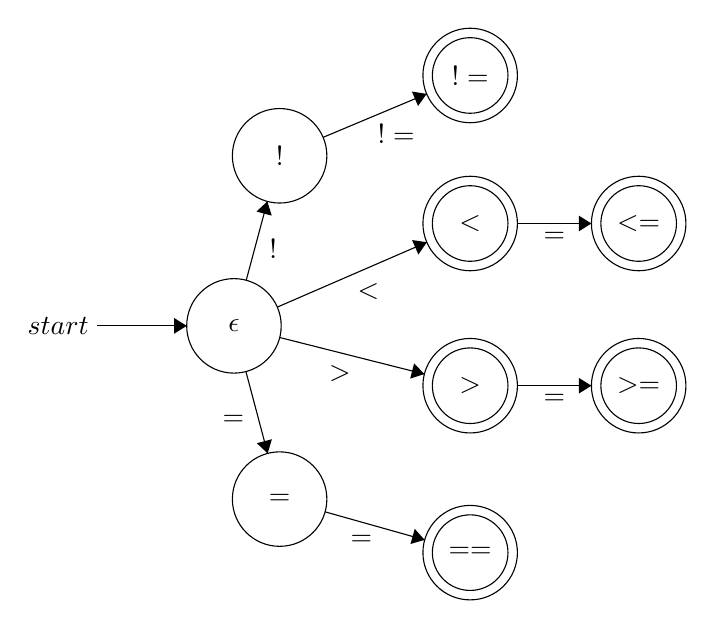
\begin{tikzpicture}[scale=0.2]
\tikzstyle{every node}+=[inner sep=0pt]
\draw [black] (45.2,-32.5) circle (3);
\draw (45.2,-32.5) node {$>=$};
\draw [black] (45.2,-32.5) circle (2.4);
\draw [black] (34.5,-22.2) circle (3);
\draw (34.5,-22.2) node {$<$};
\draw [black] (34.5,-22.2) circle (2.4);
\draw [black] (34.5,-32.5) circle (3);
\draw (34.5,-32.5) node {$>$};
\draw [black] (34.5,-32.5) circle (2.4);
\draw [black] (19.5,-28.7) circle (3);
\draw (19.5,-28.7) node {$\epsilon$};
\draw [black] (45.2,-22.2) circle (3);
\draw (45.2,-22.2) node {$<=$};
\draw [black] (45.2,-22.2) circle (2.4);
\draw [black] (22.4,-17.9) circle (3);
\draw (22.4,-17.9) node {$!$};
\draw [black] (34.5,-12.8) circle (3);
\draw (34.5,-12.8) node {$!=$};
\draw [black] (34.5,-12.8) circle (2.4);
\draw [black] (22.4,-39.7) circle (3);
\draw (22.4,-39.7) node {$=$};
\draw [black] (34.5,-43.1) circle (3);
\draw (34.5,-43.1) node {$==$};
\draw [black] (34.5,-43.1) circle (2.4);
\draw [black] (10.8,-28.7) -- (16.5,-28.7);
\draw (10.3,-28.7) node [left] {$start$};
\fill [black] (16.5,-28.7) -- (15.7,-28.2) -- (15.7,-29.2);
\draw [black] (22.25,-27.51) -- (31.75,-23.39);
\fill [black] (31.75,-23.39) -- (30.81,-23.25) -- (31.21,-24.17);
\draw (28.04,-25.96) node [below] {$<$};
\draw [black] (22.41,-29.44) -- (31.59,-31.76);
\fill [black] (31.59,-31.76) -- (30.94,-31.08) -- (30.69,-32.05);
\draw (26.22,-31.17) node [below] {$>$};
\draw [black] (37.5,-32.5) -- (42.2,-32.5);
\fill [black] (42.2,-32.5) -- (41.4,-32) -- (41.4,-33);
\draw (39.85,-33) node [below] {$=$};
\draw [black] (37.5,-22.2) -- (42.2,-22.2);
\fill [black] (42.2,-22.2) -- (41.4,-21.7) -- (41.4,-22.7);
\draw (39.85,-22.7) node [below] {$=$};
\draw [black] (20.28,-25.8) -- (21.62,-20.8);
\fill [black] (21.62,-20.8) -- (20.93,-21.44) -- (21.9,-21.7);
\draw (21.72,-23.81) node [right] {$!$};
\draw [black] (25.16,-16.73) -- (31.74,-13.97);
\fill [black] (31.74,-13.97) -- (30.8,-13.82) -- (31.19,-14.74);
\draw (29.8,-15.87) node [below] {$!=$};
\draw [black] (20.26,-31.6) -- (21.64,-36.8);
\fill [black] (21.64,-36.8) -- (21.91,-35.9) -- (20.95,-36.15);
\draw (20.19,-34.7) node [left] {$=$};
\draw [black] (25.29,-40.51) -- (31.61,-42.29);
\fill [black] (31.61,-42.29) -- (30.98,-41.59) -- (30.71,-42.55);
\draw (27.6,-41.96) node [below] {$=$};
\end{tikzpicture}
\end{center}

\section{Problem 2}

\subsection{a}

\begin{center}
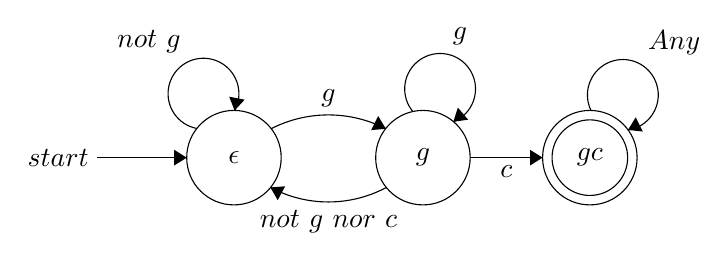
\begin{tikzpicture}[scale=0.2]
\tikzstyle{every node}+=[inner sep=0pt]
\draw [black] (19.6,-28.5) circle (3);
\draw (19.6,-28.5) node {$\epsilon$};
\draw [black] (31.6,-28.5) circle (3);
\draw (31.6,-28.5) node {$g$};
\draw [black] (42.2,-28.5) circle (3);
\draw (42.2,-28.5) node {$gc$};
\draw [black] (42.2,-28.5) circle (2.4);
\draw [black] (10.9,-28.5) -- (16.6,-28.5);
\draw (10.4,-28.5) node [left] {$start$};
\fill [black] (16.6,-28.5) -- (15.8,-28) -- (15.8,-29);
\draw [black] (42.278,-25.513) arc (206.24146:-81.75854:2.25);
\draw (47.55,-22.02) node [above] {$Any$};
\fill [black] (44.62,-26.74) -- (45.56,-26.84) -- (45.11,-25.94);
\draw [black] (34.6,-28.5) -- (39.2,-28.5);
\fill [black] (39.2,-28.5) -- (38.4,-28) -- (38.4,-29);
\draw (36.9,-29) node [below] {$c$};
\draw [black] (21.953,-26.667) arc (117.16614:62.83386:7.989);
\fill [black] (29.25,-26.67) -- (28.76,-25.86) -- (28.31,-26.75);
\draw (25.6,-25.29) node [above] {$g$};
\draw [black] (30.967,-25.58) arc (219.96376:-68.03624:2.25);
\draw (33.96,-21.38) node [above] {$g$};
\fill [black] (33.53,-26.22) -- (34.47,-26.09) -- (33.82,-25.32);
\draw [black] (29.291,-30.386) arc (-61.7765:-118.2235:7.804);
\fill [black] (21.91,-30.39) -- (22.38,-31.2) -- (22.85,-30.32);
\draw (25.6,-31.81) node [below] {$not\mbox{ }g\mbox{ }nor\mbox{ }c$};
\draw [black] (17.254,-26.649) arc (259.46335:-28.53665:2.25);
\draw (14.2,-21.89) node [above] {$not\mbox{ }g$};
\fill [black] (19.64,-25.51) -- (20.28,-24.82) -- (19.3,-24.63);
\end{tikzpicture}
\end{center}

\subsection{b}
\begin{center}
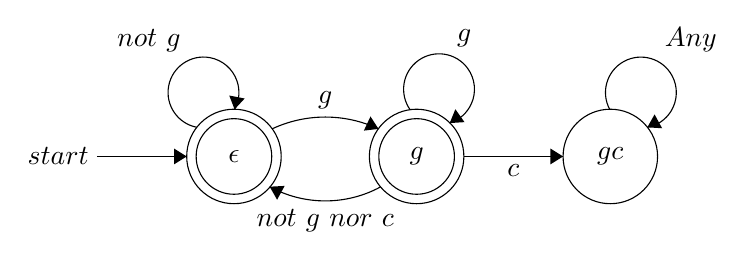
\begin{tikzpicture}[scale=0.2]
\tikzstyle{every node}+=[inner sep=0pt]
\draw [black] (19.6,-28.5) circle (3);
\draw (19.6,-28.5) node {$\epsilon$};
\draw [black] (19.6,-28.5) circle (2.4);
\draw [black] (31.2,-28.5) circle (3);
\draw (31.2,-28.5) node {$g$};
\draw [black] (31.2,-28.5) circle (2.4);
\draw [black] (43.5,-28.5) circle (3);
\draw (43.5,-28.5) node {$gc$};
\draw [black] (10.9,-28.5) -- (16.6,-28.5);
\draw (10.4,-28.5) node [left] {$start$};
\fill [black] (16.6,-28.5) -- (15.8,-28) -- (15.8,-29);
\draw [black] (17.254,-26.649) arc (259.46335:-28.53665:2.25);
\draw (14.2,-21.89) node [above] {$not\mbox{ }g$};
\fill [black] (19.64,-25.51) -- (20.28,-24.82) -- (19.3,-24.63);
\draw [black] (30.793,-25.54) arc (215.56505:-72.43495:2.25);
\draw (34.23,-21.56) node [above] {$g$};
\fill [black] (33.3,-26.38) -- (34.24,-26.32) -- (33.66,-25.5);
\draw [black] (22.016,-26.751) arc (115.11721:64.88279:7.973);
\fill [black] (28.78,-26.75) -- (28.27,-25.96) -- (27.85,-26.86);
\draw (25.4,-25.5) node [above] {$g$};
\draw [black] (28.926,-30.425) arc (-61.41463:-118.58537:7.369);
\fill [black] (21.87,-30.42) -- (22.34,-31.25) -- (22.82,-30.37);
\draw (25.4,-31.82) node [below] {$not\mbox{ }g\mbox{ }nor\mbox{ }c$};
\draw [black] (43.463,-25.512) arc (208.44003:-79.55997:2.25);
\draw (48.61,-21.9) node [above] {$Any$};
\fill [black] (45.85,-26.65) -- (46.79,-26.71) -- (46.31,-25.83);
\draw [black] (34.2,-28.5) -- (40.5,-28.5);
\fill [black] (40.5,-28.5) -- (39.7,-28) -- (39.7,-29);
\draw (37.35,-29) node [below] {$c$};
\end{tikzpicture}
\end{center}

\subsection{c}

Labels are in the form of $a/t$ where $e=$even and $o=$odd.

\begin{center}
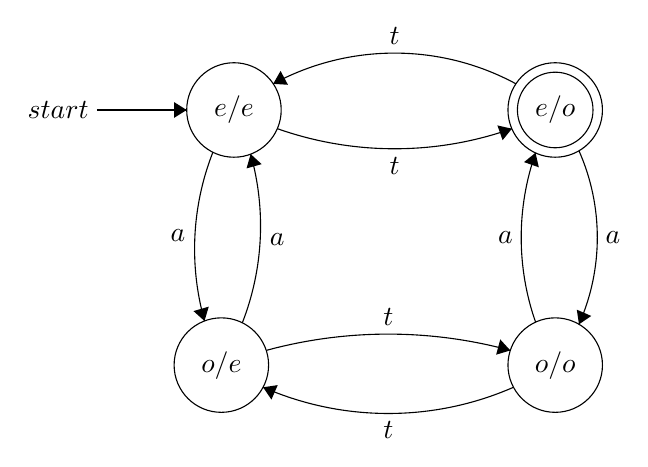
\begin{tikzpicture}[scale=0.2]
\tikzstyle{every node}+=[inner sep=0pt]
\draw [black] (13,-20.7) circle (3);
\draw (13,-20.7) node {$e/e$};
\draw [black] (33.4,-20.7) circle (3);
\draw (33.4,-20.7) node {$e/o$};
\draw [black] (33.4,-20.7) circle (2.4);
\draw [black] (12.2,-36.9) circle (3);
\draw (12.2,-36.9) node {$o/e$};
\draw [black] (33.4,-36.9) circle (3);
\draw (33.4,-36.9) node {$o/o$};
\draw [black] (4.3,-20.7) -- (10,-20.7);
\draw (3.8,-20.7) node [left] {$start$};
\fill [black] (10,-20.7) -- (9.2,-20.2) -- (9.2,-21.2);
\draw [black] (30.647,-21.886) arc (-70.53364:-109.46636:22.346);
\fill [black] (30.65,-21.89) -- (29.73,-21.68) -- (30.06,-22.62);
\draw (23.2,-23.66) node [below] {$t$};
\draw [black] (15.492,-19.038) arc (118.39896:61.60104:16.206);
\fill [black] (15.49,-19.04) -- (16.43,-19.1) -- (15.96,-18.22);
\draw (23.2,-16.59) node [above] {$t$};
\draw [black] (34.907,-23.287) arc (23.89585:-23.89585:13.609);
\fill [black] (34.91,-34.31) -- (35.69,-33.78) -- (34.77,-33.38);
\draw (36.57,-28.8) node [right] {$a$};
\draw [black] (32.154,-34.176) arc (-160.70402:-199.29598:16.268);
\fill [black] (32.15,-23.42) -- (31.42,-24.01) -- (32.36,-24.34);
\draw (30.74,-28.8) node [left] {$a$};
\draw [black] (11.133,-34.101) arc (-164.23512:-201.41913:16.832);
\fill [black] (11.13,-34.1) -- (11.4,-33.19) -- (10.43,-33.47);
\draw (9.95,-28.68) node [left] {$a$};
\draw [black] (14.061,-23.502) arc (15.66621:-21.32046:16.91);
\fill [black] (14.06,-23.5) -- (13.8,-24.41) -- (14.76,-24.14);
\draw (15.24,-28.92) node [right] {$a$};
\draw [black] (15.05,-35.967) arc (105.21342:74.78658:29.534);
\fill [black] (30.55,-35.97) -- (29.91,-35.27) -- (29.65,-36.24);
\draw (22.8,-34.43) node [above] {$t$};
\draw [black] (30.754,-38.307) arc (-66.33845:-113.66155:19.818);
\fill [black] (14.85,-38.31) -- (15.38,-39.09) -- (15.78,-38.17);
\draw (22.8,-40.47) node [below] {$t$};
\end{tikzpicture}
\end{center}

\subsection{d}

\begin{center}
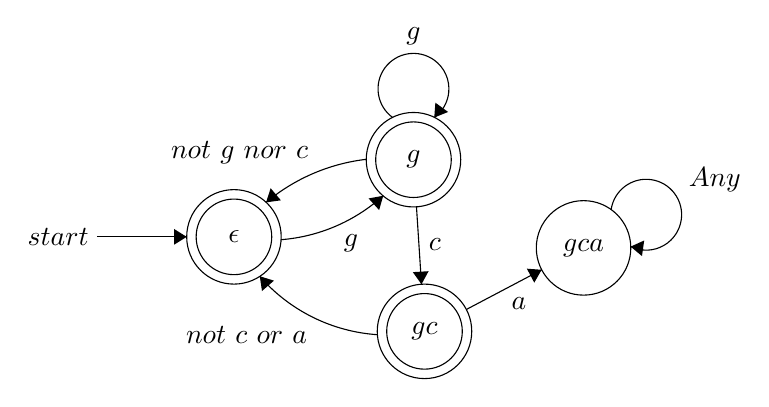
\begin{tikzpicture}[scale=0.2]
\tikzstyle{every node}+=[inner sep=0pt]
\draw [black] (13.6,-20.7) circle (3);
\draw (13.6,-20.7) node {$\epsilon$};
\draw [black] (13.6,-20.7) circle (2.4);
\draw [black] (25,-15.8) circle (3);
\draw (25,-15.8) node {$g$};
\draw [black] (25,-15.8) circle (2.4);
\draw [black] (25.7,-26.7) circle (3);
\draw (25.7,-26.7) node {$gc$};
\draw [black] (25.7,-26.7) circle (2.4);
\draw [black] (35.8,-21.4) circle (3);
\draw (35.8,-21.4) node {$gca$};
\draw [black] (4.9,-20.7) -- (10.6,-20.7);
\draw (4.4,-20.7) node [left] {$start$};
\fill [black] (10.6,-20.7) -- (9.8,-20.2) -- (9.8,-21.2);
\draw [black] (37.55,-18.977) arc (171.89727:-116.10273:2.25);
\draw (42.45,-17.08) node [right] {$Any$};
\fill [black] (38.79,-21.32) -- (39.51,-21.92) -- (39.65,-20.93);
\draw [black] (23.076,-18.09) arc (-47.89679:-85.58477:10.937);
\fill [black] (23.08,-18.09) -- (22.15,-18.26) -- (22.82,-19);
\draw (21.03,-20.54) node [below] {$g$};
\draw [black] (23.677,-13.12) arc (234:-54:2.25);
\draw (25,-8.55) node [above] {$g$};
\fill [black] (26.32,-13.12) -- (27.2,-12.77) -- (26.39,-12.18);
\draw [black] (15.641,-18.512) arc (129.8965:96.62195:12.102);
\fill [black] (15.64,-18.51) -- (16.58,-18.38) -- (15.93,-17.61);
\draw (13.96,-16.12) node [above] {$not\mbox{ }g\mbox{ }nor\mbox{ }c$};
\draw [black] (25.19,-18.79) -- (25.51,-23.71);
\fill [black] (25.51,-23.71) -- (25.96,-22.88) -- (24.96,-22.94);
\draw (25.94,-21.21) node [right] {$c$};
\draw [black] (22.717,-26.913) arc (-93.80603:-138.94463:10.879);
\fill [black] (15.24,-23.2) -- (15.38,-24.14) -- (16.14,-23.48);
\draw (14.4,-26.33) node [below] {$not\mbox{ }c\mbox{ }or\mbox{ }a$};
\draw [black] (28.36,-25.31) -- (33.14,-22.79);
\fill [black] (33.14,-22.79) -- (32.2,-22.72) -- (32.67,-23.61);
\draw (31.69,-24.55) node [below] {$a$};
\end{tikzpicture}
\end{center}

\section{Problem 3}

\begin{center}
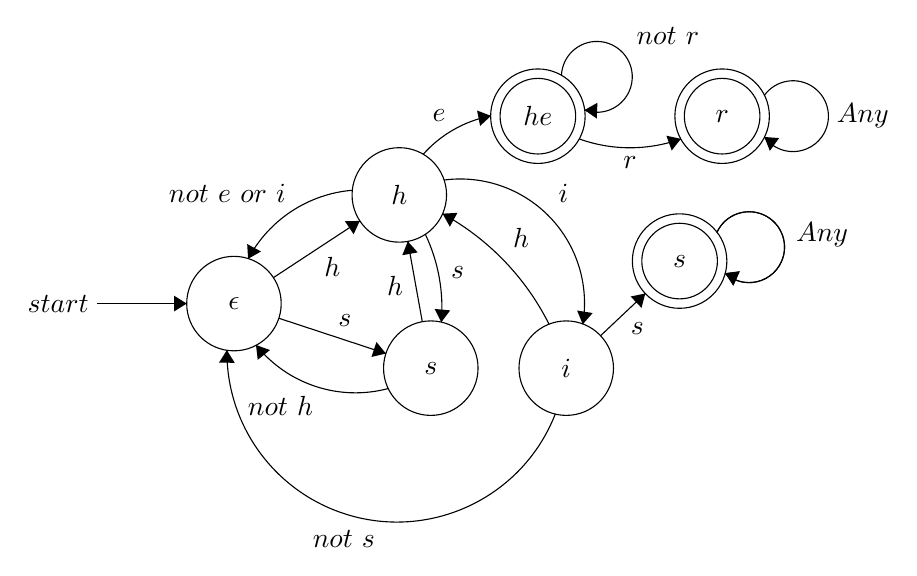
\begin{tikzpicture}[scale=0.2]
\tikzstyle{every node}+=[inner sep=0pt]
\draw [black] (13.6,-20.7) circle (3);
\draw (13.6,-20.7) node {$\epsilon$};
\draw [black] (24.1,-13.8) circle (3);
\draw (24.1,-13.8) node {$h$};
\draw [black] (26.1,-24.8) circle (3);
\draw (26.1,-24.8) node {$s$};
\draw [black] (32.9,-8.8) circle (3);
\draw (32.9,-8.8) node {$he$};
\draw [black] (32.9,-8.8) circle (2.4);
\draw [black] (34.7,-24.8) circle (3);
\draw (34.7,-24.8) node {$i$};
\draw [black] (41.9,-18) circle (3);
\draw (41.9,-18) node {$s$};
\draw [black] (41.9,-18) circle (2.4);
\draw [black] (44.6,-8.8) circle (3);
\draw (44.6,-8.8) node {$r$};
\draw [black] (44.6,-8.8) circle (2.4);
\draw [black] (4.9,-20.7) -- (10.6,-20.7);
\draw (4.4,-20.7) node [left] {$start$};
\fill [black] (10.6,-20.7) -- (9.8,-20.2) -- (9.8,-21.2);
\draw [black] (16.45,-21.63) -- (23.25,-23.87);
\fill [black] (23.25,-23.87) -- (22.65,-23.14) -- (22.33,-24.09);
\draw (20.64,-22.22) node [above] {$s$};
\draw [black] (25.56,-21.85) -- (24.64,-16.75);
\fill [black] (24.64,-16.75) -- (24.29,-17.63) -- (25.27,-17.45);
\draw (24.38,-19.57) node [left] {$h$};
\draw [black] (16.11,-19.05) -- (21.59,-15.45);
\fill [black] (21.59,-15.45) -- (20.65,-15.47) -- (21.2,-16.3);
\draw (19.85,-17.75) node [below] {$h$};
\draw [black] (25.609,-11.229) arc (138.40912:100.79978:7.689);
\fill [black] (29.92,-8.78) -- (29.04,-8.44) -- (29.23,-9.42);
\draw (26.62,-9.15) node [above] {$e$};
\draw [black] (26.929,-12.856) arc (97.56994:-9.69176:7.893);
\fill [black] (35.75,-22.01) -- (36.38,-21.3) -- (35.39,-21.14);
\draw (34.18,-13.73) node [right] {$i$};
\draw [black] (36.88,-22.74) -- (39.72,-20.06);
\fill [black] (39.72,-20.06) -- (38.79,-20.25) -- (39.48,-20.97);
\draw (39.21,-21.88) node [below] {$s$};
\draw [black] (44.268,-16.178) arc (155.30993:-132.69007:2.25);
\draw (49.26,-16.36) node [right] {$Any$};
\fill [black] (44.79,-18.77) -- (45.31,-19.56) -- (45.72,-18.65);
\draw [black] (44.268,-16.178) arc (155.30993:-132.69007:2.25);
\fill [black] (44.79,-18.77) -- (45.31,-19.56) -- (45.72,-18.65);
\draw [black] (34.396,-6.213) arc (177.69223:-110.30777:2.25);
\draw (39.13,-3.72) node [right] {$not\mbox{ }r$};
\fill [black] (35.86,-8.41) -- (36.64,-8.95) -- (36.68,-7.95);
\draw [black] (14.505,-17.857) arc (151.95329:94.66797:8.271);
\fill [black] (14.5,-17.86) -- (15.32,-17.39) -- (14.44,-16.92);
\draw (13.18,-14.33) node [above] {$not\mbox{ }e\mbox{ }or\mbox{ }i$};
\draw [black] (23.411,-26.091) arc (-74.98078:-141.3382:8.086);
\fill [black] (15,-23.33) -- (15.11,-24.27) -- (15.89,-23.65);
\draw (16.56,-26.56) node [below] {$not\mbox{ }h$};
\draw [black] (34.006,-27.709) arc (-21.3727:-180.61985:10.798);
\fill [black] (13.15,-23.66) -- (12.65,-24.45) -- (13.65,-24.46);
\draw (20.58,-35.09) node [below] {$not\mbox{ }s$};
\draw [black] (25.75,-16.294) arc (25.5323:-4.92261:10.817);
\fill [black] (26.77,-21.88) -- (27.33,-21.13) -- (26.34,-21.04);
\draw (27.36,-18.76) node [right] {$s$};
\draw [black] (26.848,-14.994) arc (61.26375:26.61443:16.36);
\fill [black] (26.85,-14.99) -- (27.31,-15.82) -- (27.79,-14.94);
\draw (31.29,-16.52) node [right] {$h$};
\draw [black] (41.983,-10.241) arc (-70.17194:-109.82806:9.531);
\fill [black] (41.98,-10.24) -- (41.06,-10.04) -- (41.4,-10.98);
\draw (38.75,-11.31) node [below] {$r$};
\draw [black] (47.28,-7.477) arc (144:-144:2.25);
\draw (51.85,-8.8) node [right] {$Any$};
\fill [black] (47.28,-10.12) -- (47.63,-11) -- (48.22,-10.19);
\end{tikzpicture}
\end{center}

\section{Problem 4}

\begin{proof}

    We will induct on the length of an input string $w$.\\

    Basis: The base case $|w| = 0$, i.e. $w = \epsilon$. In this case, $\delta(0, w) = 0$\\. This holds with the language definition.

    Inductive: Let $w=xa$ be a string where $a$ is the last symbol of $w$ and $x$ is the string the precedes $a$. The inductive hypothesis holds for
    $x$. We must consider the transitions that might occur based on what state, $S$, that the automaton ended on when given the input $x$.\\

    Assume that $S=0$. There are two possible transitions out of this state. In the case where $a$ is 0, we are essentially multiplying the binary
    integer by 2. Multiplying an integer that is divisible by 3 by 2 yields another integer that is divisible by 3. Therefore, the language definition
    holds. In the case when $a$ is 1, this has the effect of adding 1 to the binary integer. Considering that the general form of an integer that is
    divisible by 3 can be represented as $3m, m \in \mathbb{R}$, then multiplying by 2 and adding 1 would yield $6m + 1$, which is not divisible by 3. In the automaton,
    this case correctly transfers for a non-accepting state, which holds with the language definition.\\

    Now consider the case where $S=1$. There are two possible transitions out of this state. Consider the transition where we add a 1 to the string. To be
    in this state, the integer would have something to the form would $6m + 1$. The addition of this 1 will have the effect of multiplying by 2 and adding 1, yielding
    an integer of the form $12m + 3$, which is divisible by 3. The addition of a 0 would have the effect of mulitplying by 2, yielding $12m + 2$, which is not divisible
    by 3. The first transition will transfer to an accepting state, which holds will the language. Similarly, the second transition will transfer to a non-accepting state,
    which also holds with the language.

    Lastly, consider the case where $S = 2$. A transition with 1 would have the effect of multiplying an integer of the form $12m + 2$ by 2 and adding 1, which yields a
    number that is not divisible by 3, and is also a non-accepting state. The transition with 0 has the effect of multiplying by 2, which yields a number not divisible by 3
    and ends at a non-accepting state. Both of these transitions hold with the definition of the language.

    Therefore, all transitions from each state in the automaton hold with the definition of the language.

\end{proof}

\section{Problem 5}
\begin{center}
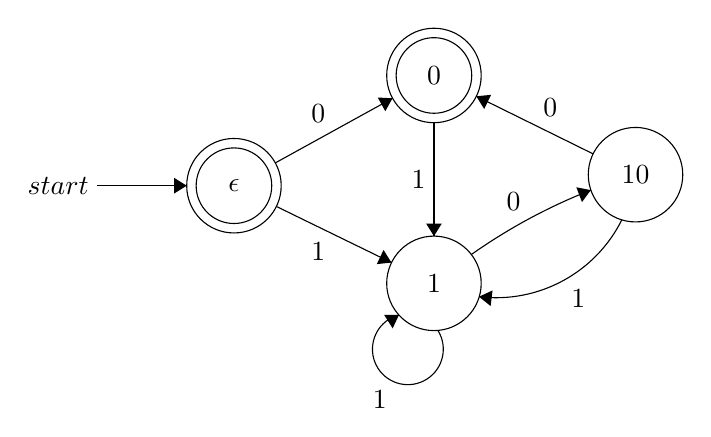
\begin{tikzpicture}[scale=0.2]
\tikzstyle{every node}+=[inner sep=0pt]
\draw [black] (13.6,-20.7) circle (3);
\draw (13.6,-20.7) node {$\epsilon$};
\draw [black] (13.6,-20.7) circle (2.4);
\draw [black] (26.3,-13.7) circle (3);
\draw (26.3,-13.7) node {$0$};
\draw [black] (26.3,-13.7) circle (2.4);
\draw [black] (26.3,-26.9) circle (3);
\draw (26.3,-26.9) node {$1$};
\draw [black] (39.1,-20) circle (3);
\draw (39.1,-20) node {$10$};
\draw [black] (4.9,-20.7) -- (10.6,-20.7);
\draw (4.4,-20.7) node [left] {$start$};
\fill [black] (10.6,-20.7) -- (9.8,-20.2) -- (9.8,-21.2);
\draw [black] (16.23,-19.25) -- (23.67,-15.15);
\fill [black] (23.67,-15.15) -- (22.73,-15.1) -- (23.21,-15.97);
\draw (18.95,-16.7) node [above] {$0$};
\draw [black] (26.3,-16.7) -- (26.3,-23.9);
\fill [black] (26.3,-23.9) -- (26.8,-23.1) -- (25.8,-23.1);
\draw (25.8,-20.3) node [left] {$1$};
\draw [black] (16.3,-22.02) -- (23.6,-25.58);
\fill [black] (23.6,-25.58) -- (23.1,-24.78) -- (22.67,-25.68);
\draw (18.96,-24.31) node [below] {$1$};
\draw [black] (38.236,-22.858) arc (-26.44333:-96.90178:8.934);
\fill [black] (29.16,-27.75) -- (29.9,-28.34) -- (30.02,-27.35);
\draw (35.47,-27.25) node [below] {$1$};
\draw [black] (26.543,-29.878) arc (32.39411:-255.60589:2.25);
\draw (22.86,-33.69) node [below] {$1$};
\fill [black] (24.08,-28.9) -- (23.14,-28.91) -- (23.68,-29.76);
\draw [black] (28.676,-25.069) arc (125.22607:111.42881:35.89);
\fill [black] (36.26,-20.98) -- (35.34,-20.8) -- (35.7,-21.74);
\draw (31.35,-22.29) node [above] {$0$};
\draw [black] (36.41,-18.68) -- (28.99,-15.02);
\fill [black] (28.99,-15.02) -- (29.49,-15.83) -- (29.93,-14.93);
\draw (33.69,-16.34) node [above] {$0$};
\end{tikzpicture}
\end{center}


\end{document}
